\documentclass[10pt]{nsibeamer}
\usepackage{animate}
\title{CH14 : \\Arbres binaires}
\author{T$^{\text{ale}}$ NSI}

\begin{document}

\maketitle
\section{Généralités}
\begin{frame}{Arbres}
    La structure d'arbre n'est pas linéaire : les éléments n'y sont pas rangés les uns à la suite des autres.\\\pause
     C'est une structure \alert{hiérarchique} : les éléments y sont organisés en \textit{niveaux}.\\\pause
    
    Dans ce chapitre nous étudions les \alert{arbres binaires}.
\end{frame}

\begin{frame}{Définition : arbre}
    Un arbre binaire peut être vide.\pause
    Sinon, il est composé d'au moins un n\oe ud, appelé \alert{racine} et le reste des n\oe uds peut être partagé en 2 sous-ensembles :\pause le \alert{sous-arbre gauche} et le \alert{sous-arbre droit}.\pause
    \begin{center}
        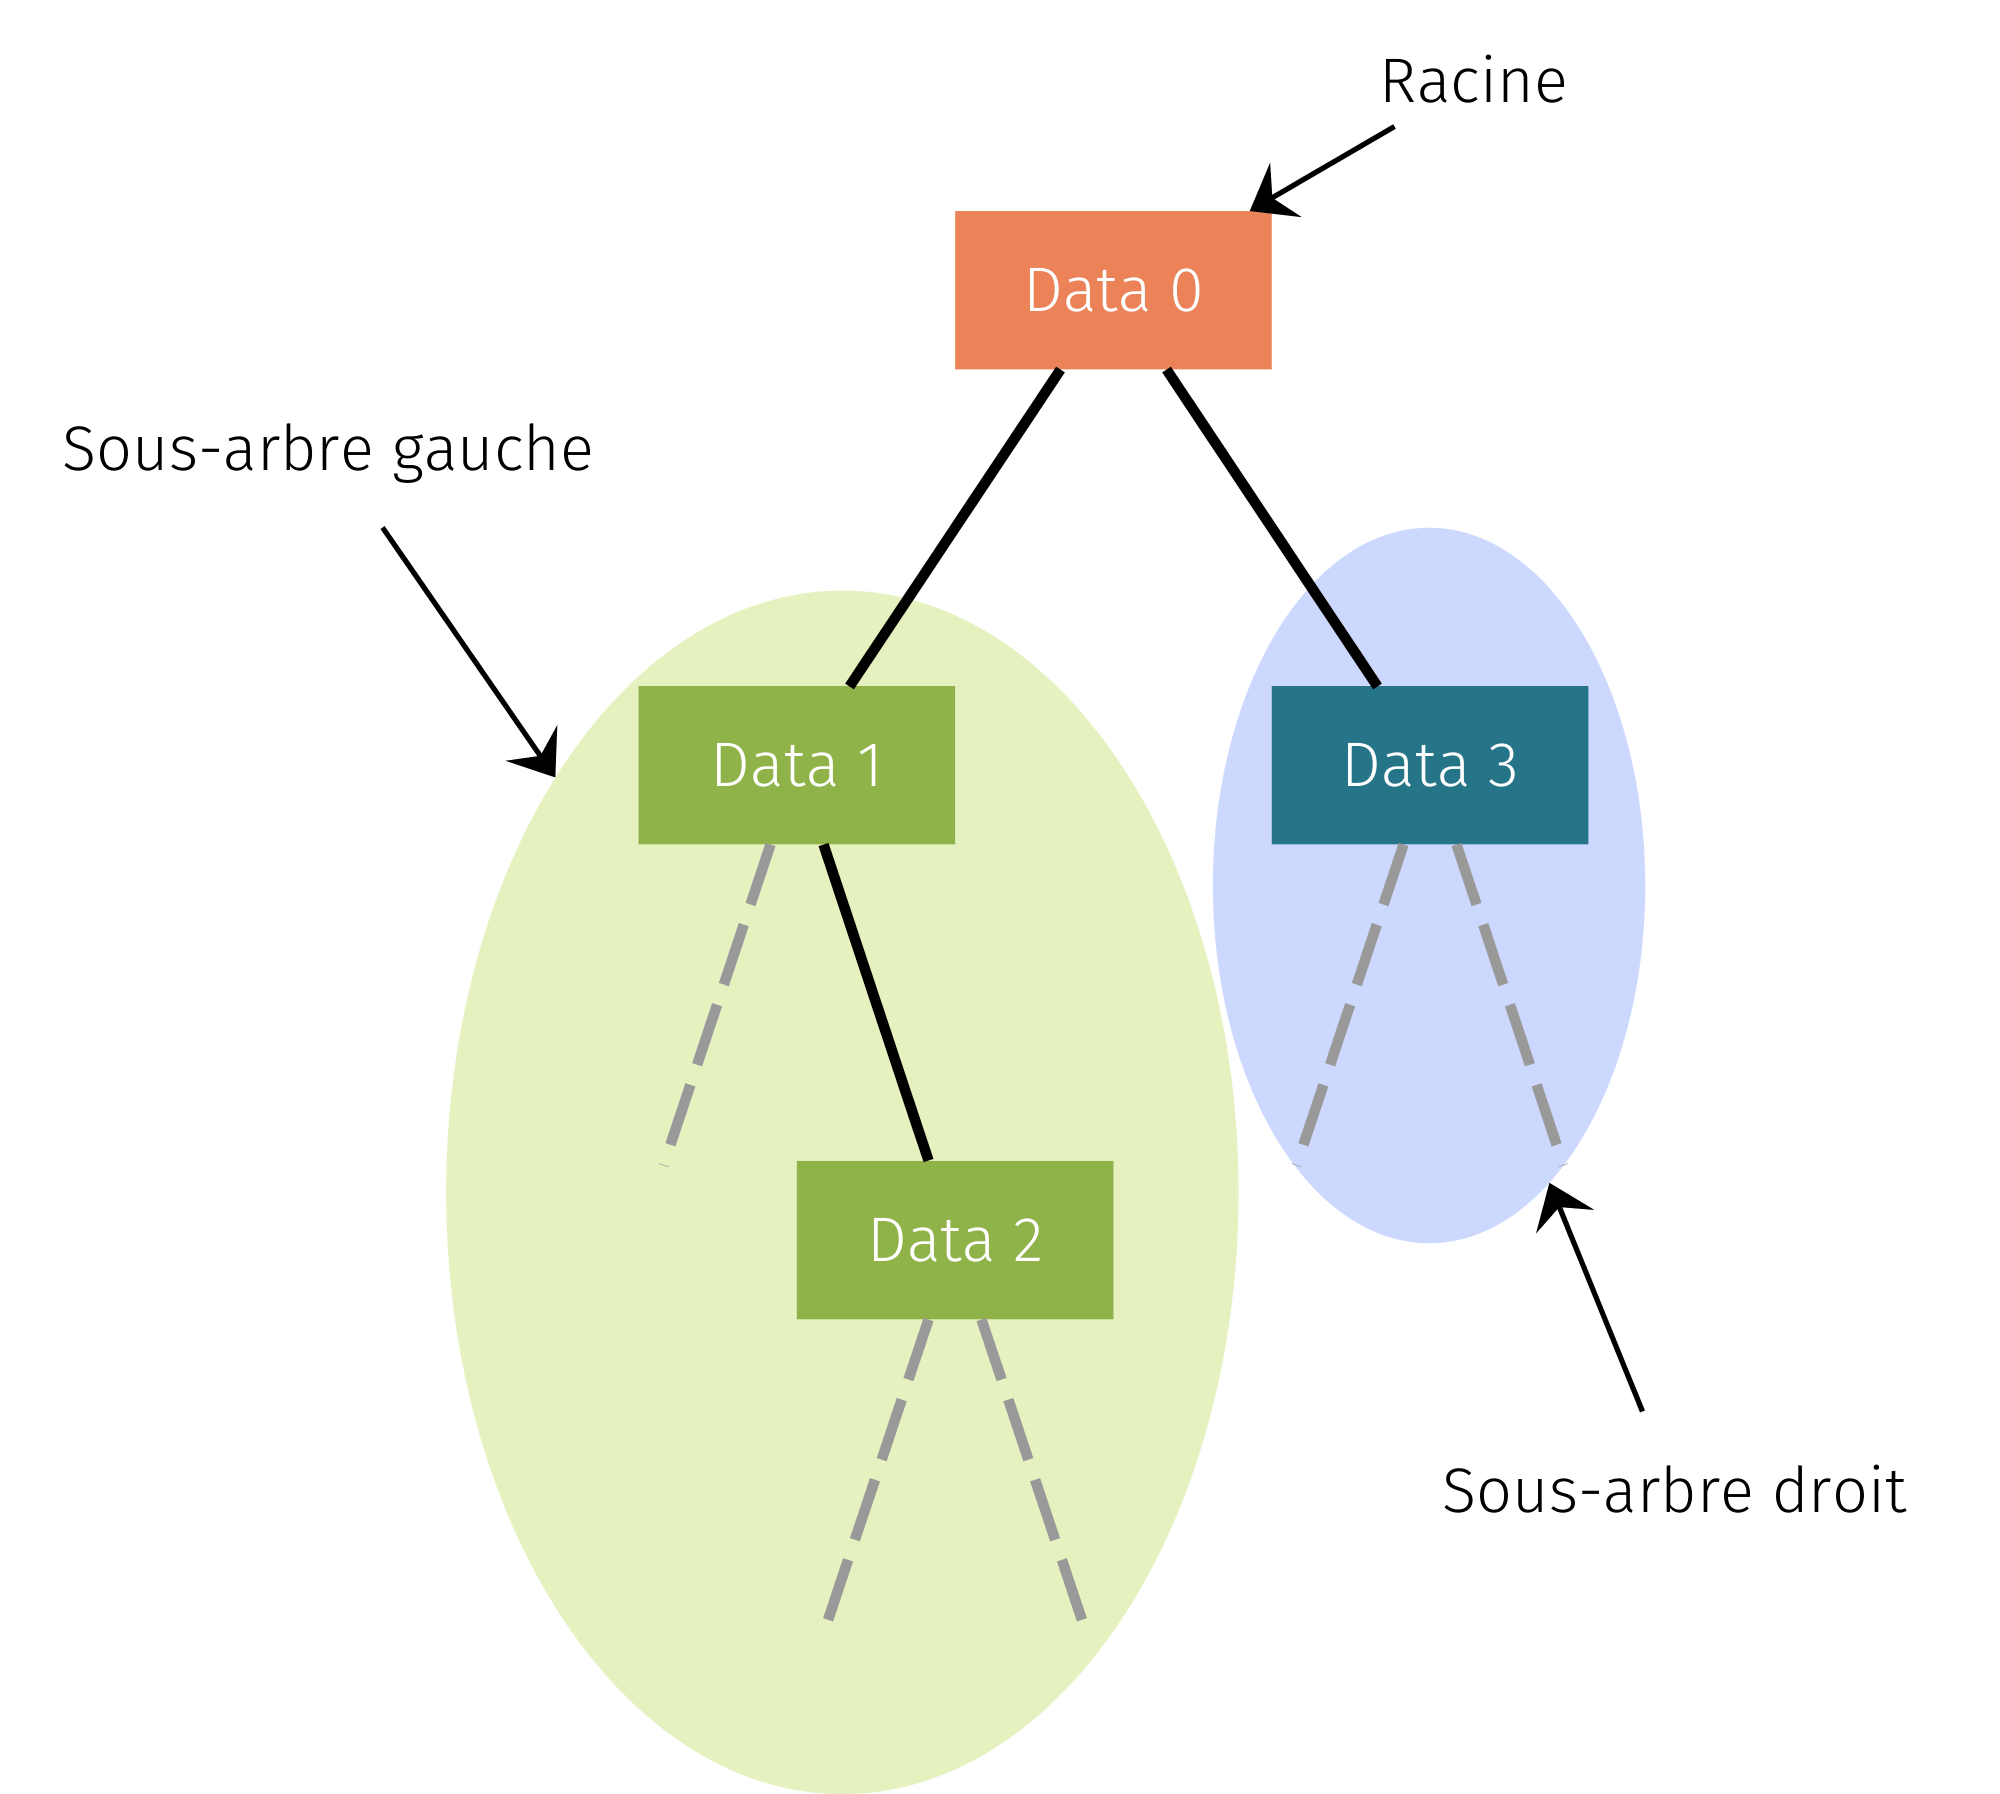
\includegraphics[width=4cm]{img/arbre_bin_1}
    \end{center}\pause
Un n\oe ud possède toujours un sous-arbre droit et un sous-arbre gauche, même si ceux-ci peuvent être vides (segments gris en pointillés).
\end{frame}

\begin{frame}{Définition}
    Quand le sous-arbre gauche d'un n\oe ud est non-vide, sa racine est appelée \alert{fils gauche} du n\oe ud. On définit de même la notion de \alert{fils droit}
    \begin{center}
        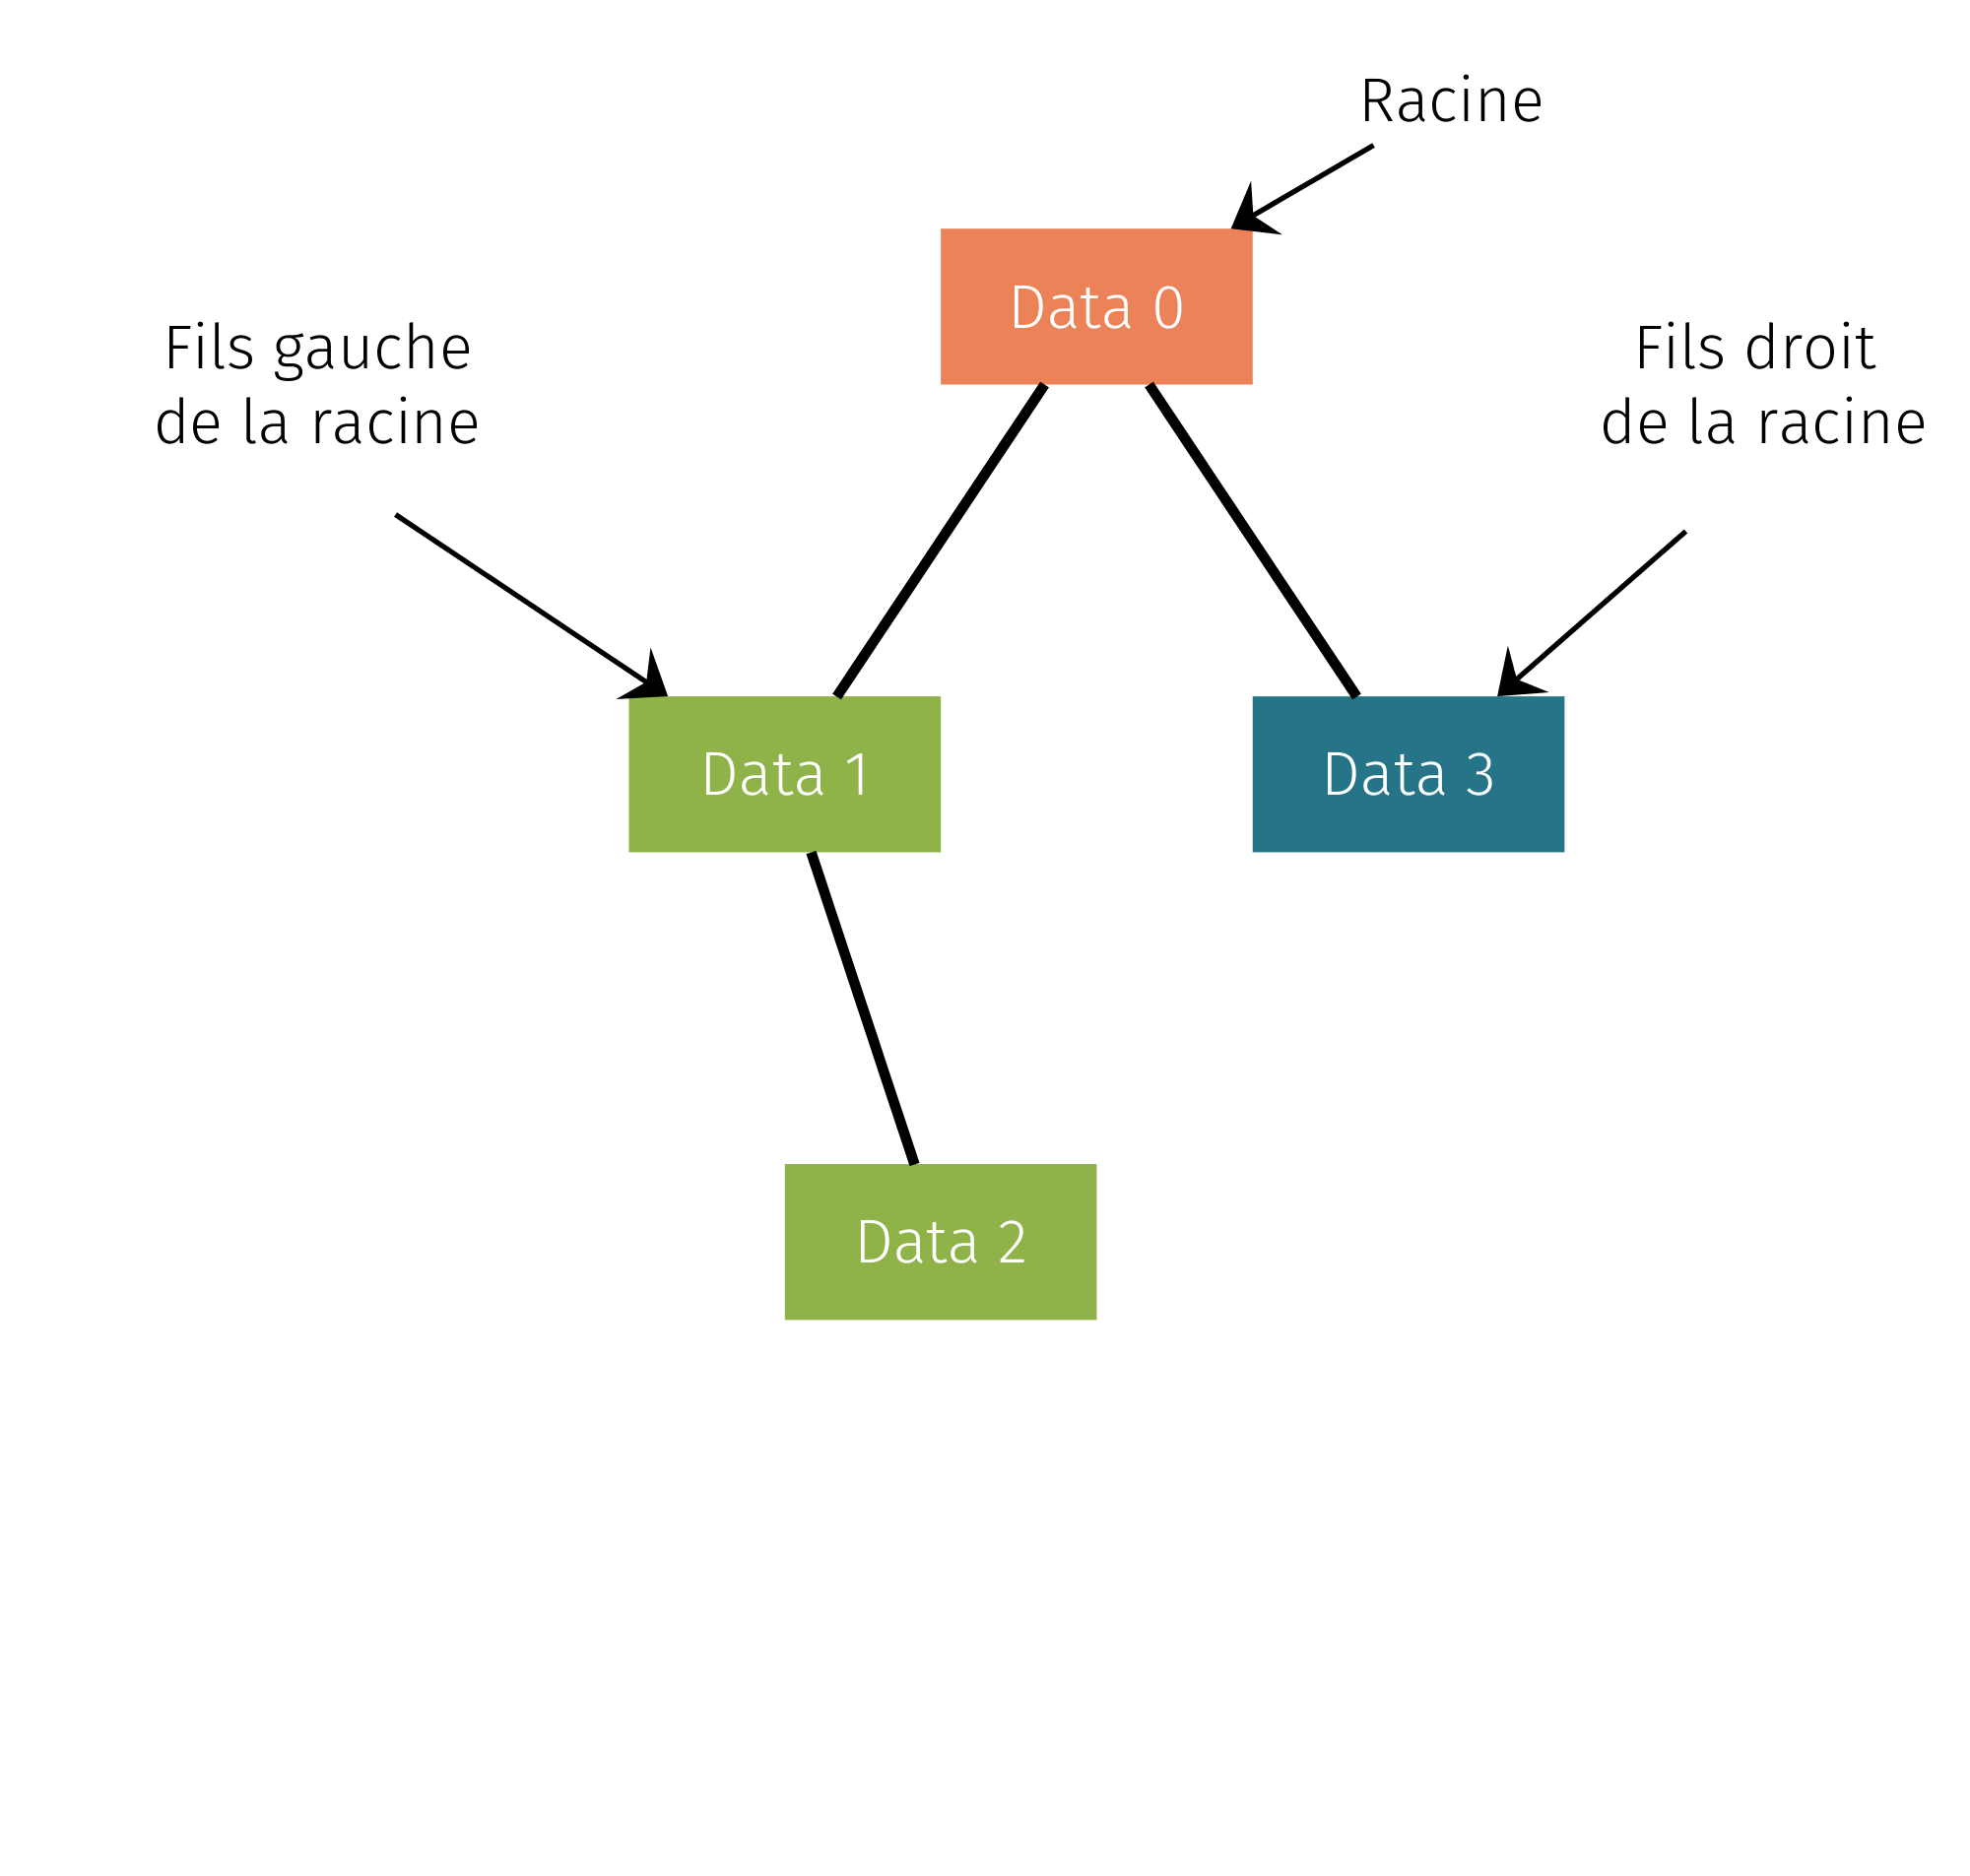
\includegraphics[width=5cm]{img/arbre_bin_2}
    \end{center}
\end{frame}

\begin{frame}{Taille}
La \alert{taille} d'un arbre est le nombre de ses n\oe uds.
    \begin{center}
    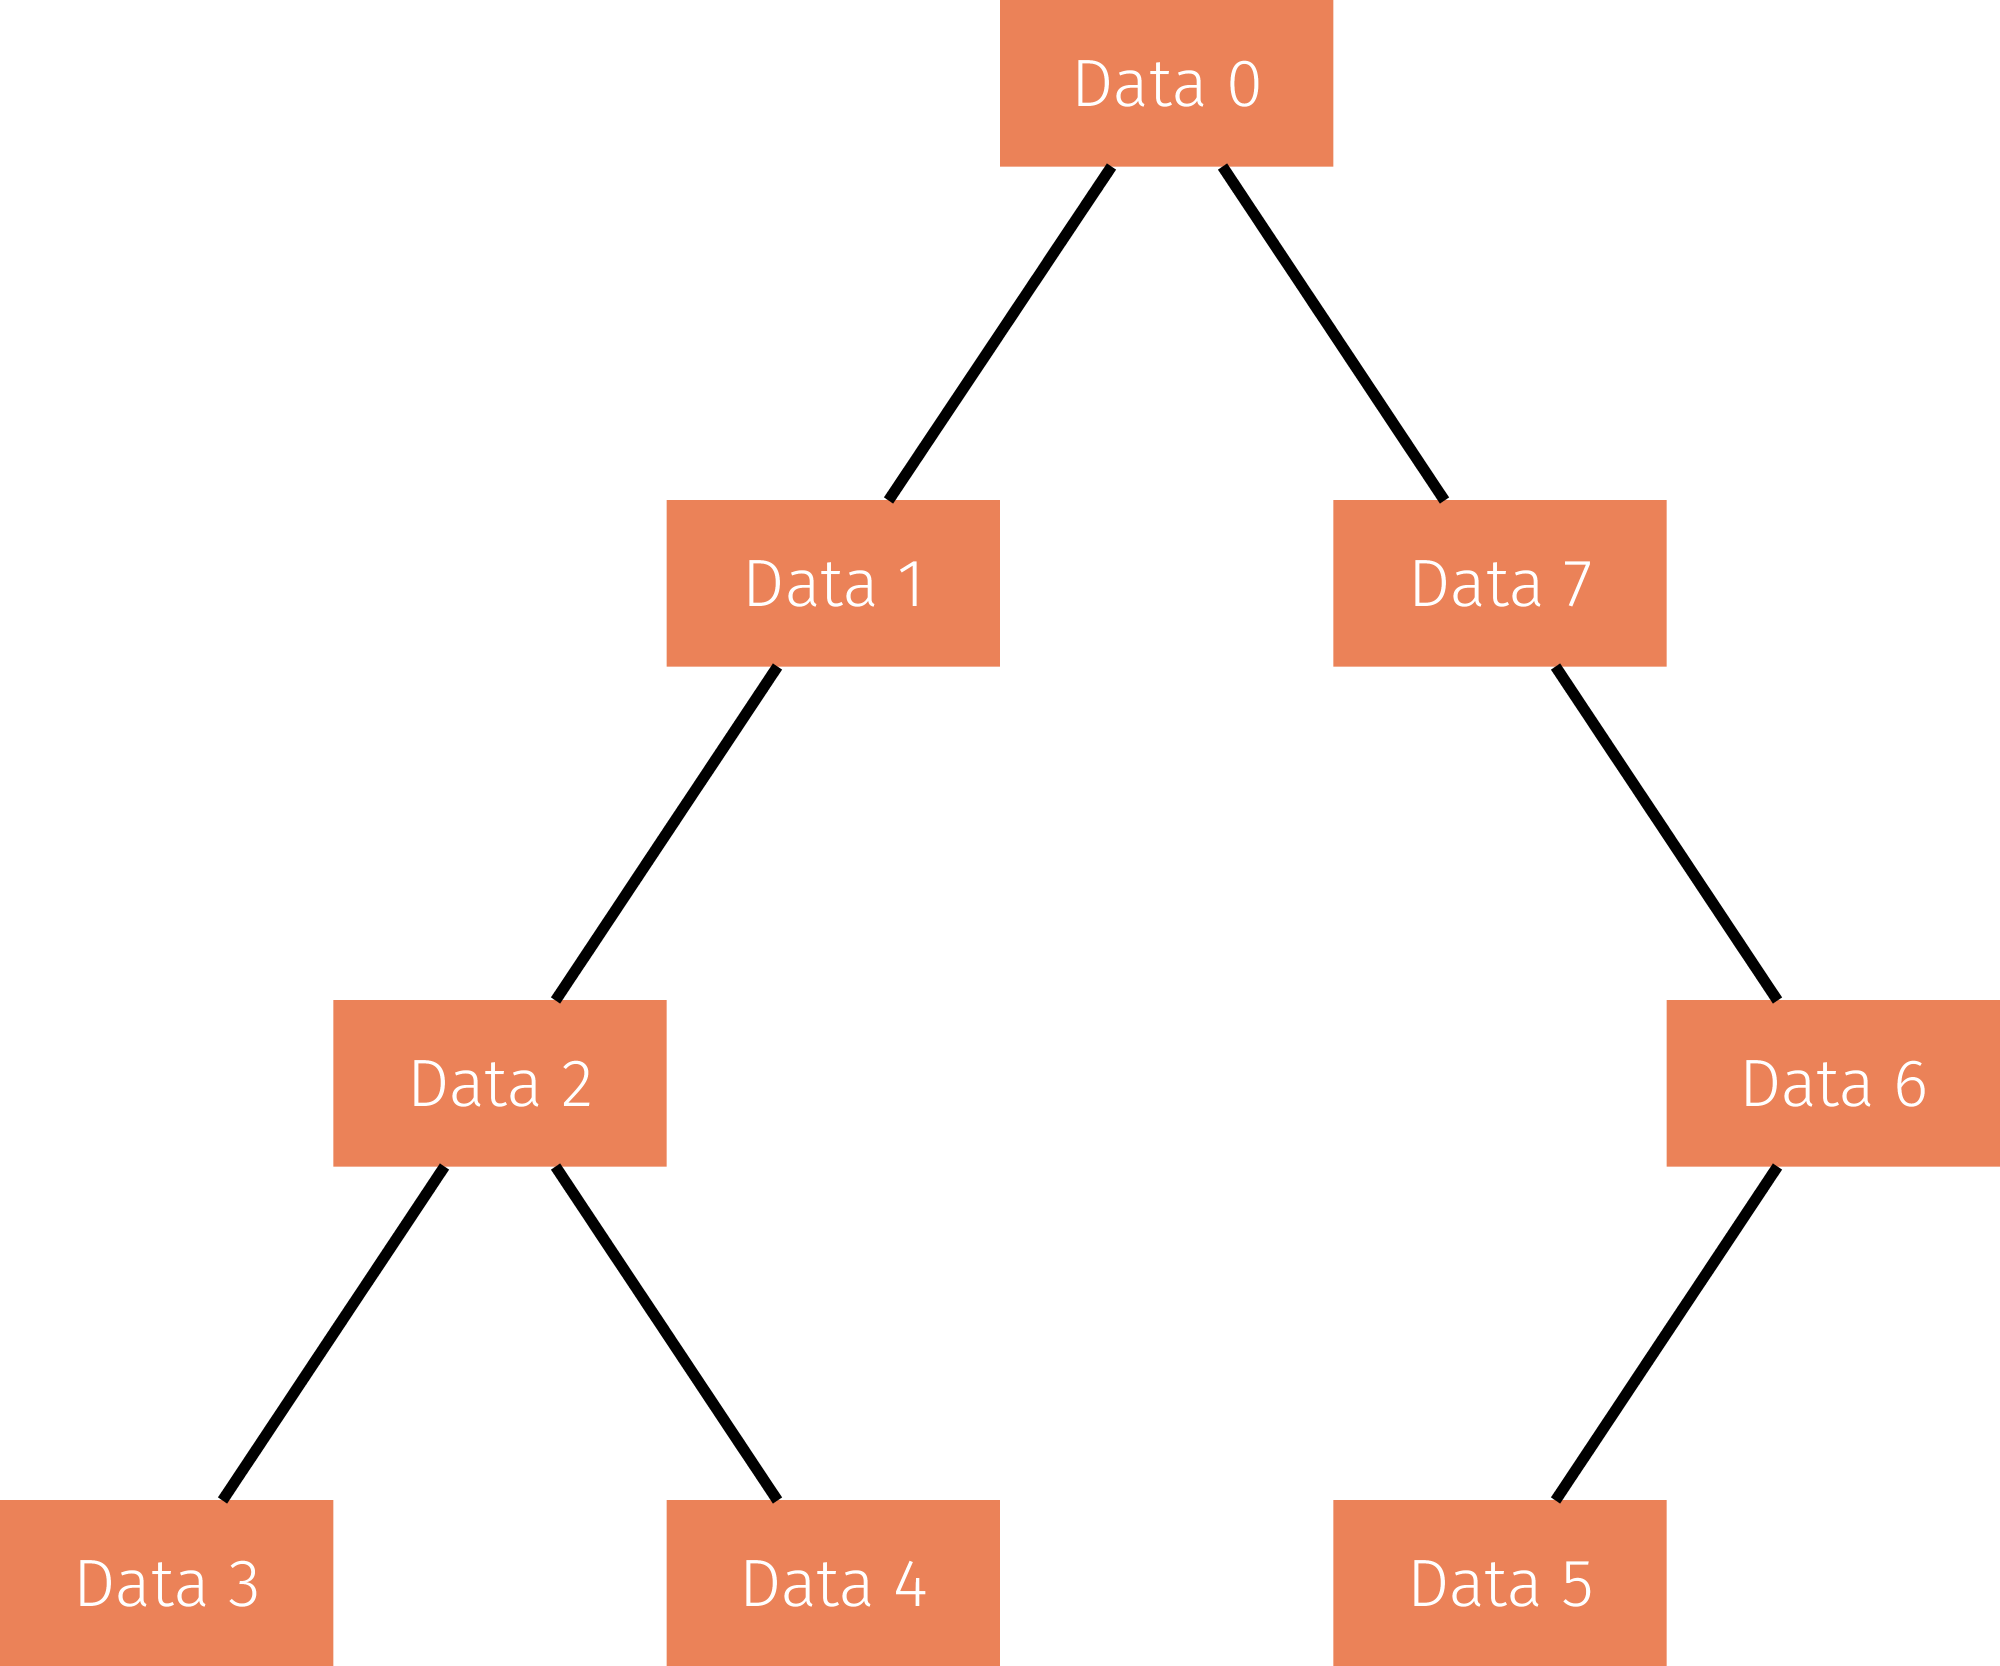
\includegraphics[width=5cm]{img/arbre_bin_5}
\end{center}
Voici un arbre de taille 8.

\end{frame}

\begin{frame}{Hauteur et feuilles}
On appelle \alert{feuille} tout n\oe ud qui n'a ni fils droit ni fils gauche.\\
    \begin{center}
    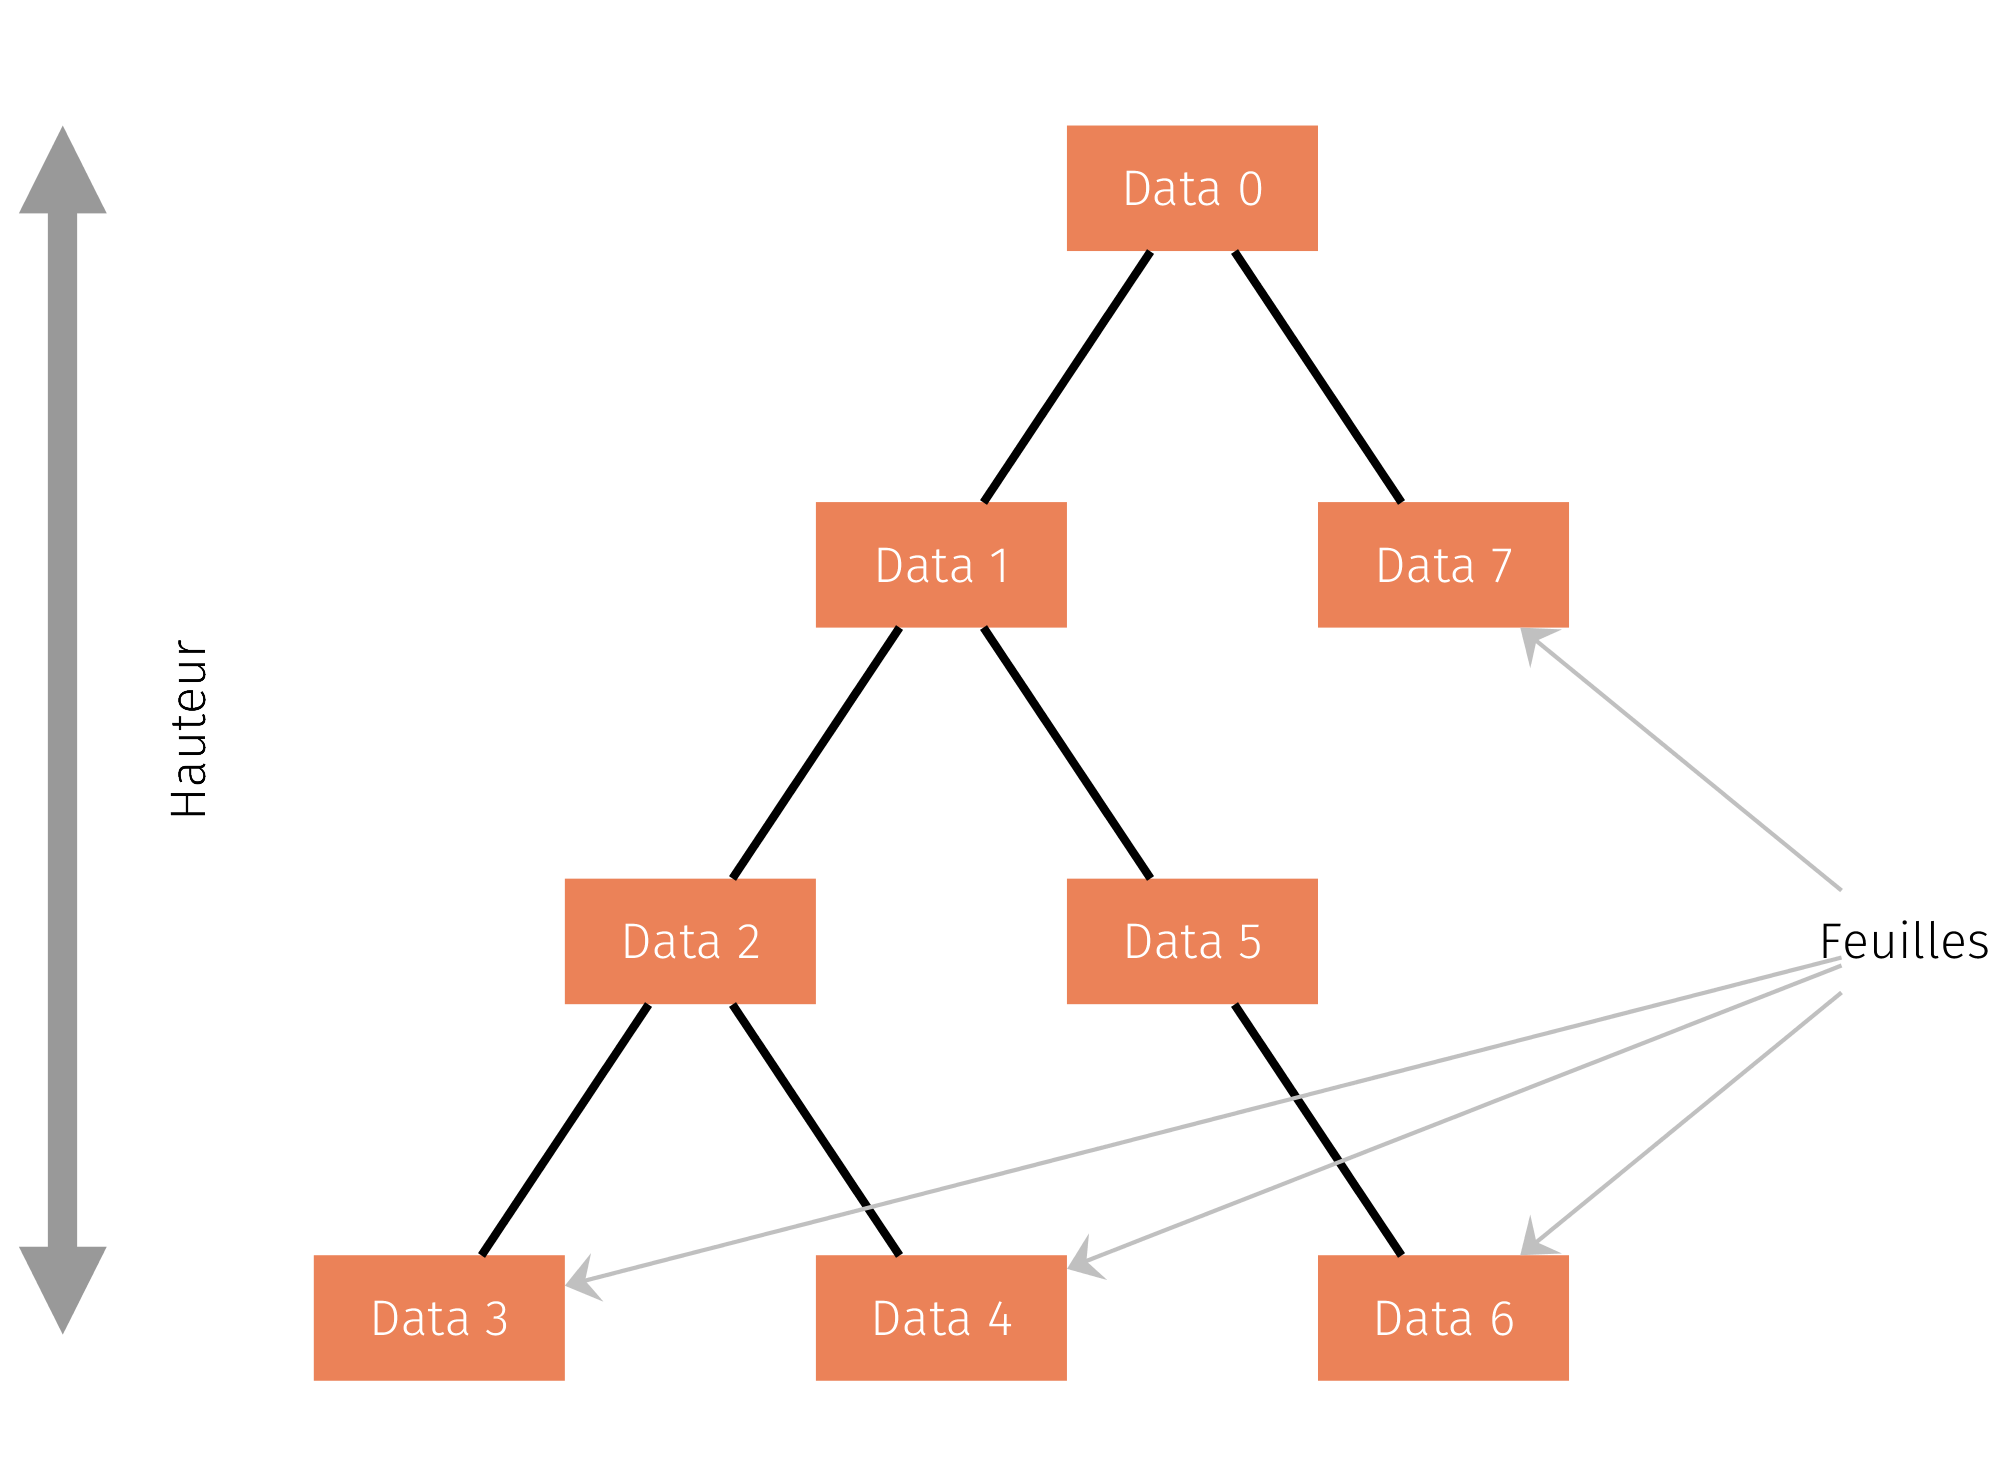
\includegraphics[width=5cm]{img/arbre_bin_3}
\end{center}\pause
La \alert{hauteur} d'un n\oe ud est le nombre d'arêtes qui mène de la racine à ce n\oe ud).\\\pause
La hauteur de l'arbre est la plus grande des hauteurs des n\oe uds qui le composent.\\\pause
Cet arbre est de hauteur 3.
\end{frame}
\begin{frame}{Remarque}
La définition de hauteur \alert{ n'est pas standard}. Selon celle-ci la hauteur de l'arbre vide n'est pas définie.\\\pause

On choisit parfois de définir la hauteur d'un n\oe ud comme le nombre de n\oe uds pour aller jusqu'à la racine incluse, et on fixe la hauteur de l'arbre vide à zéro.\\

Cela donne une hauteur qui est supérieure d'une unité par rapport à celle choisie dans ce cours.\pause
\end{frame}

\begin{frame}{N\oe ud interne}
Un n\oe ud qui n'est ni la racine ni une feuille est dit \alert{interne}.\pause
    \begin{center}
    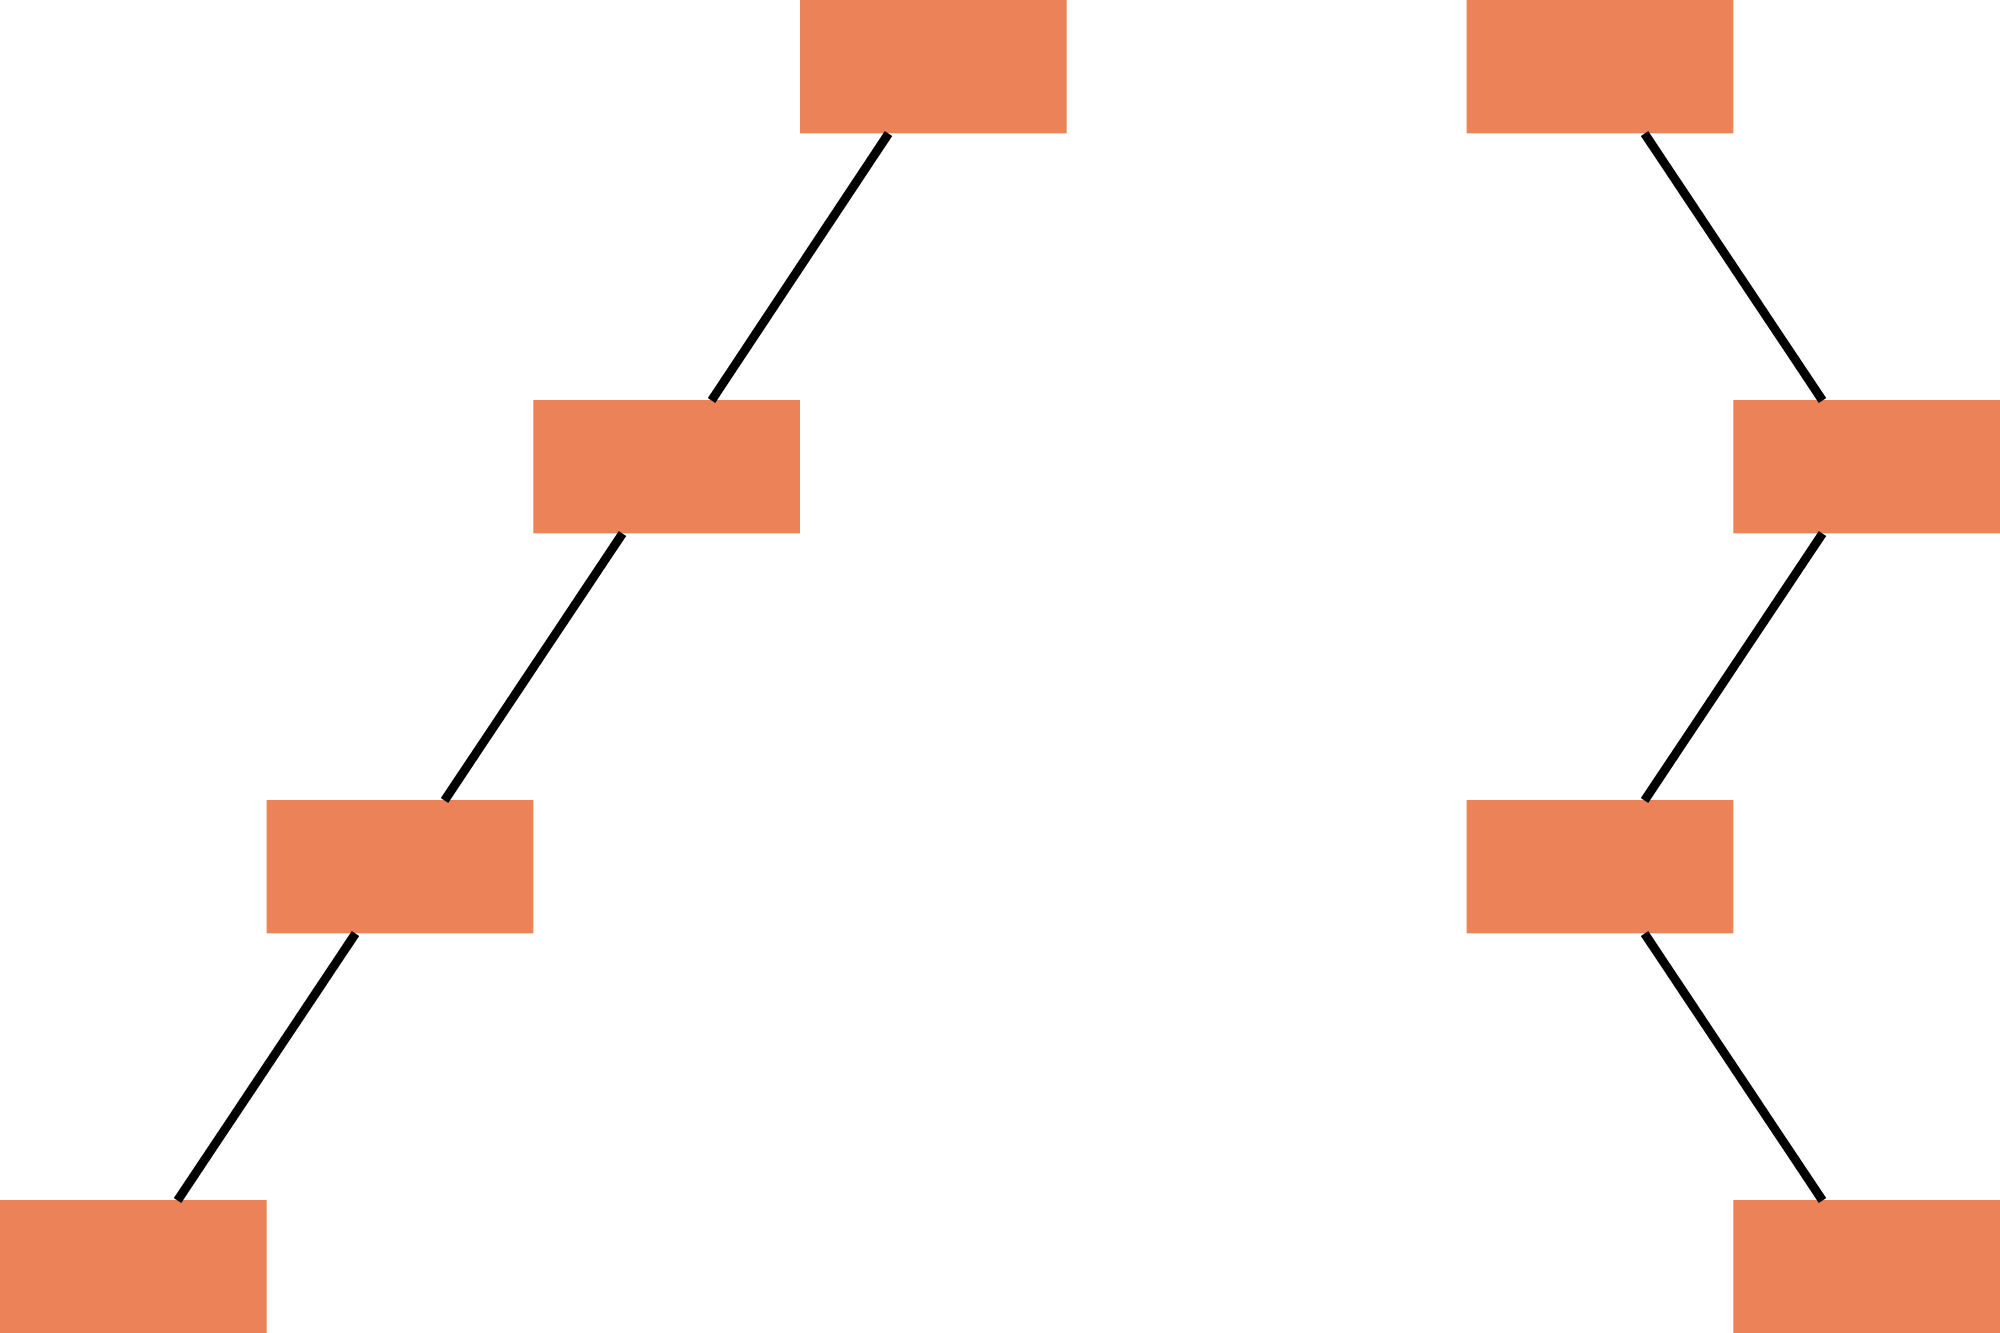
\includegraphics[width=5cm]{img/peigne}
\end{center}
Si tous les n\oe uds internes n'ont qu'un seul fils, l'arbre est dit \alert{dégénéré}.
\end{frame}

\begin{frame}{Arbres parfaits}
    Si tous les n\oe uds internes ont 2 fils et que toutes les feuilles sont à la même hauteur, on dit que l'arbre binaire est \alert{parfait}.
    \begin{center}
        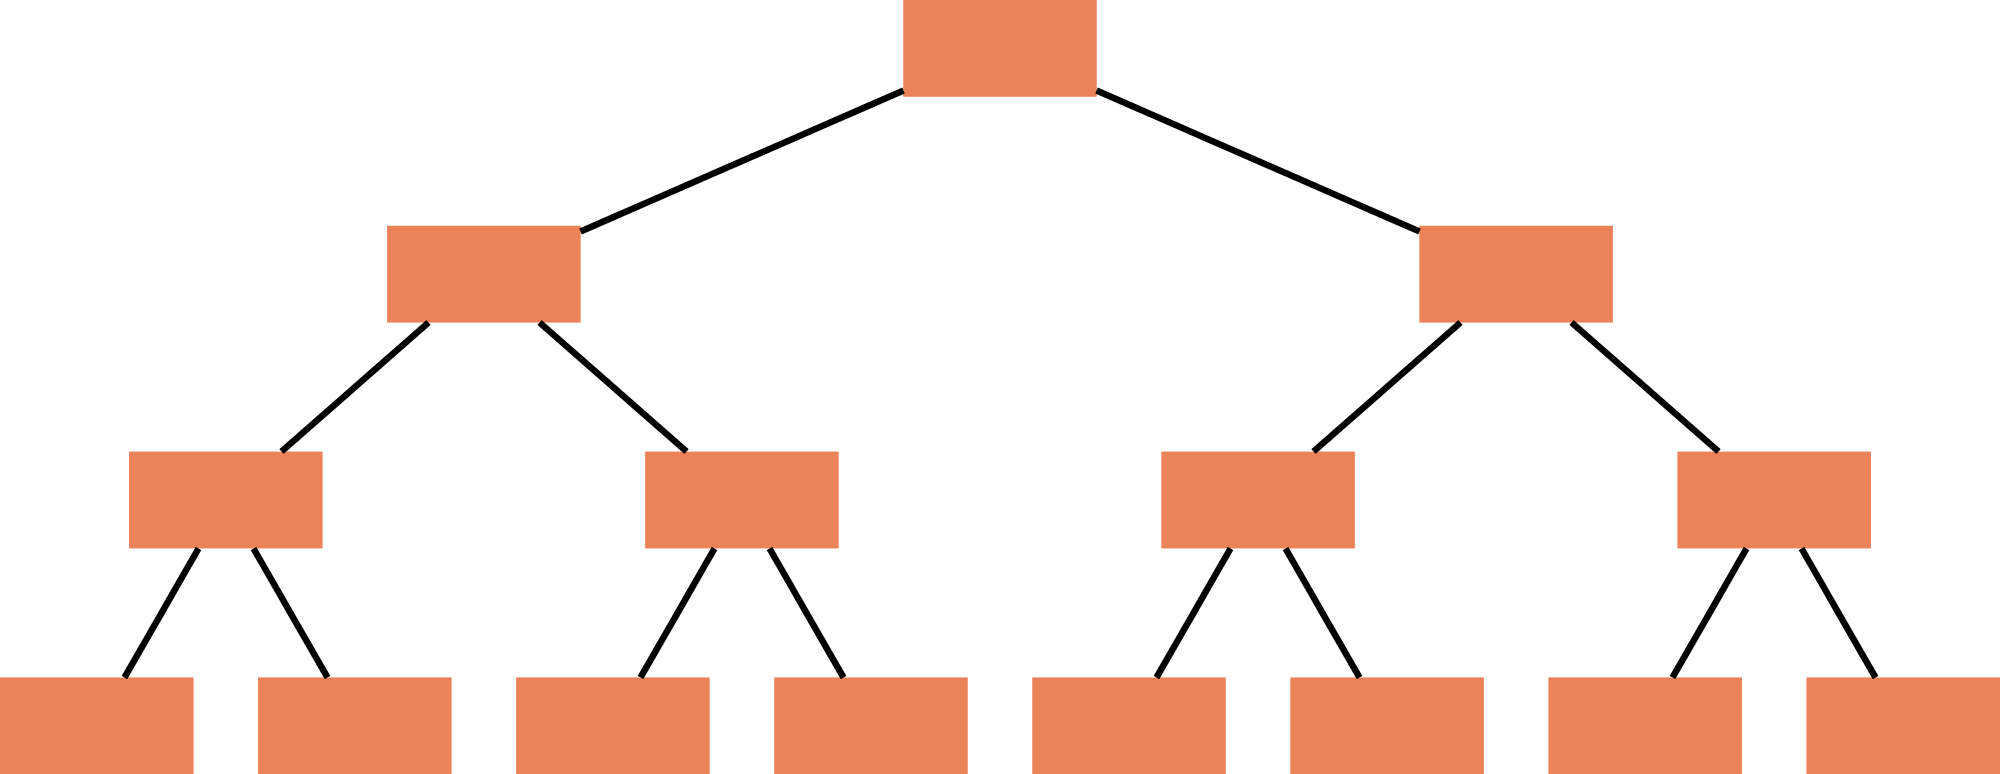
\includegraphics[width=6cm]{img/parfait}
    \end{center}
\end{frame}
\section{Structure de données}
\begin{frame}{Modèle théorique de l'arbre}
    \begin{itemize}
        \item \textit{arbre\_vide()} : crée un arbre binaire vide\pause
        \item \textit{racine(arbre)} : renvoie le n\oe ud qui est la racine de l'arbre\pause
        \item  \textit{gauche(arbre)} : renvoie le sous-arbre gauche de l'arbre\pause
        \item  \textit{droit(arbre)} : renvoie le sous-arbre droit de l'arbre\pause
        \item \textit{contenu(n\oe ud)} : renvoie l'élément stocké dans le n\oe ud\pause
    \end{itemize}
On ne suivra pas complètement ce modèle théorique.
\end{frame}

\begin{frame}[fragile]{Implémentation en Python}
\begin{minted}[fontsize=\small]{python}
class Node:
    def __init__(self, value, left=None, right=None):
        self.value = value
        self.left = left  # left child
        self.right = right  # right child
\end{minted}


\pause
Dans ce modèle on ne définit que la classe \mintinline{python}{Node}. \mintinline{python}{Node(2)} renvoie un n\oe ud sans fils droit ni fils gauche contenant la valeur 2.
\end{frame}
\begin{frame}[fragile]{Exemple}
Ce code :
\begin{minted}{python}
>>> l = Node('Data1')
>>> r = Node('Data2')
>>> root = Node('Data0', l, r)
\end{minted}
\pause
Produit ceci : 
    \begin{center}
    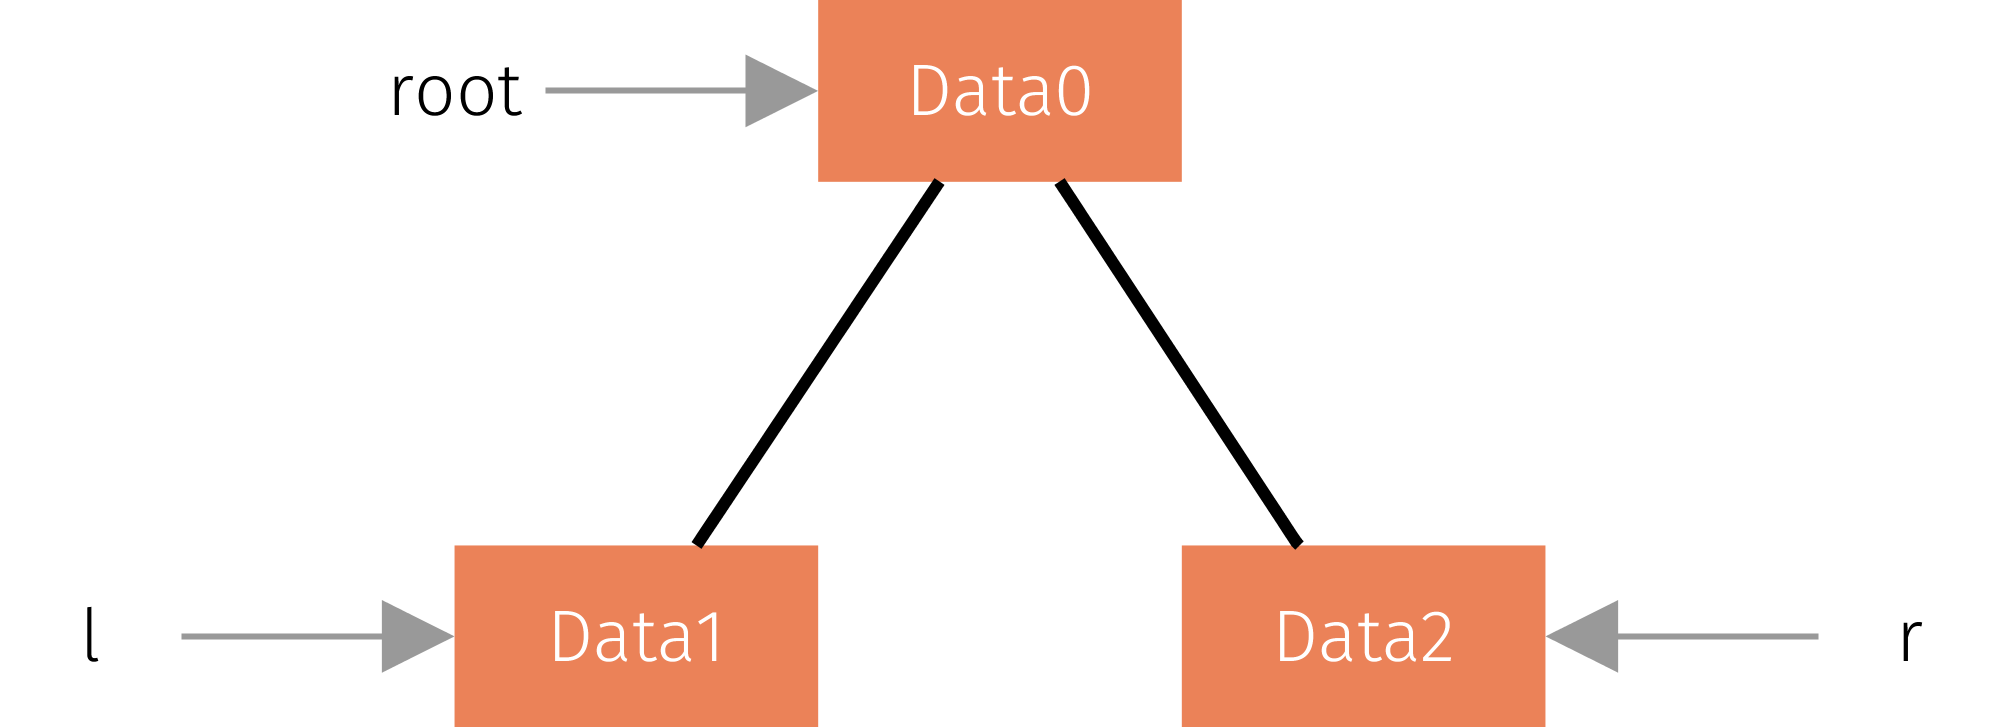
\includegraphics[width=6cm]{img/arbre_bin_4}
\end{center}
\end{frame}
\begin{frame}{Remarque}
Une instance de la classe \mintinline{python}{Node} contient 
\begin{enumerate}[--]
	\item une valeur;
    \item 2 références à 2 autres instances de la classe \mintinline{python}{Node} (ou bien \mintinline{python}{None}).
\end{enumerate}  \pause
Tout comme les listes chaînées, les arbres sont des structures qui se prêtent bien à la récursivité.
\end{frame}
\begin{frame}{Exemple}
    La taille de l'arbre vide est 0, sinon c'est « 1 plus la taille du sous-arbre gauche plus la taille du sous-arbre droit».\pause
    \begin{center}
        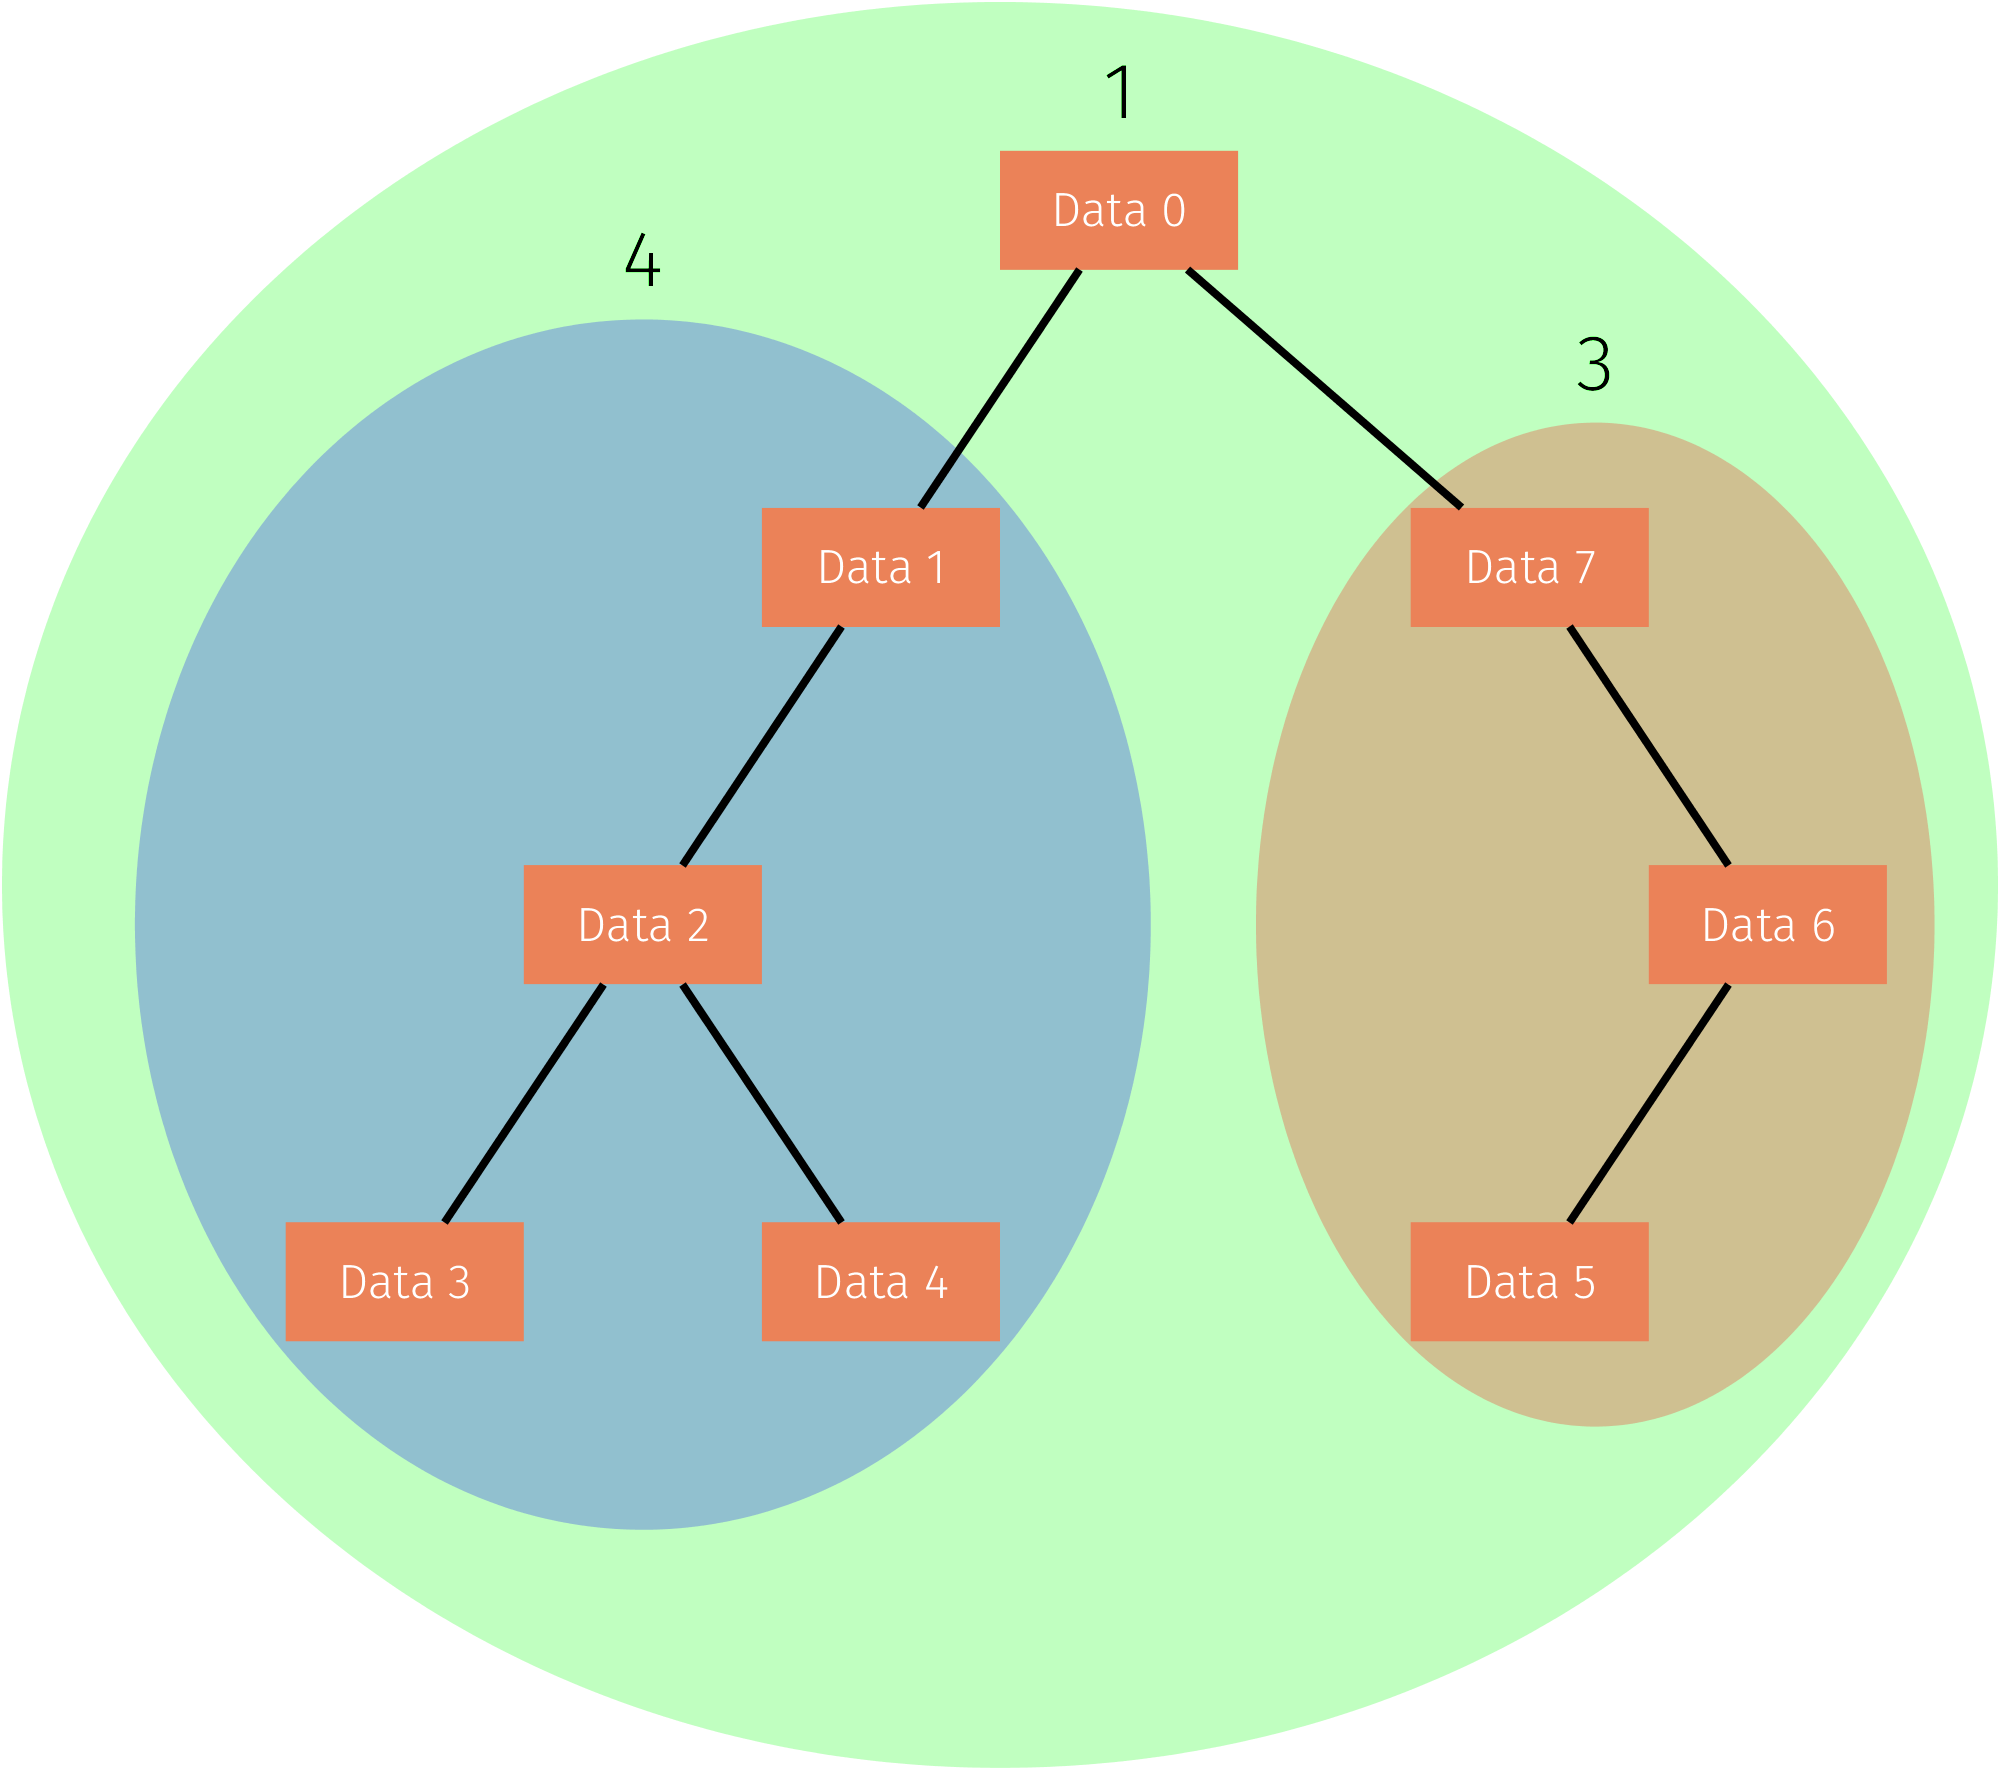
\includegraphics[width=5.5cm]{img/taille}
    \end{center}
La taille de cet arbre est 1 + 4 + 3 = 8.
\end{frame}
\section{Parcours}
\begin{frame}{Différents parcours}
Pour parcourir un arbre binaire, on peut utiliser diverses méthodes récursives.\\
Parmi celles-ci, il en existe qui consistent à\\ 
\begin{itemize}
    \item traiter le n\oe ud courant;\\
    \item parcourir le sous arbre gauche s'il est non vide;\\
    \item parcourir le sous-arbre droit s'il est non vide.\\
\end{itemize}
Et ceci \alert{dans un ordre donné}.\\
Si on choisit de toujours parcourir le sous-arbre gauche avant le droit, cela nous donne 3 méthodes.
\end{frame}
\begin{frame}{préfixe, infixe, postfixe}
\begin{itemize}
    \item \textbf{Parcours préfixe :} Traiter d'abord le n\oe ud courant puis ensuite parcourir le sous-arbre gauche, puis le droit.\pause
    \item \textbf{Parcours infixe :} Parcourir d'abord le  sous-arbre gauche, puis traiter le n\oe ud courant et ensuite parcourir le sous-arbre le droit.\pause
    \item  \textbf{Parcours postfixe :} Parcourir d'abord les sous-arbres gauche et droit puis traiter le n\oe ud courant.
\end{itemize}
\end{frame}

\begin{frame}{Parcours préfixe}
    \begin{center}
        \animategraphics[step,width=6cm]{0.2}{img/prefixe/prefixe}{0}{18}
    \end{center}
\end{frame}
\begin{frame}{Parcours infixe}
    \begin{center}
        \animategraphics[step,width=6cm]{0.2}{img/infixe/infixe}{0}{18}
    \end{center}
\end{frame}
\begin{frame}{Parcours postfixe}
    \begin{center}
        \animategraphics[step,width=6cm]{0.2}{img/postfixe/postfixe}{0}{18}
    \end{center}
\end{frame}

\end{document}